\documentclass[problem]{mcs}

\begin{pcomments}
  \pcomment{PS_four_door_random_or_not}
  \pcomment{extends CP_the_four_door_deal}
  \pcomment{added by njoliat 4/22/11 based on Fall10 problem}
\end{pcomments}

\pkeywords{
  probability
  Monty_Hall
  tree_diagram
}

%%%%%%%%%%%%%%%%%%%%%%%%%%%%%%%%%%%%%%%%%%%%%%%%%%%%%%%%%%%%%%%%%%%%%
% Problem starts here
%%%%%%%%%%%%%%%%%%%%%%%%%%%%%%%%%%%%%%%%%%%%%%%%%%%%%%%%%%%%%%%%%%%%%

% S09

\begin{problem}

Let's see what happens when \emph{Let's Make a Deal} is played with
\textbf{four} doors.  A prize is hidden behind one of the four
doors. Then the contestant picks a door.  Next, the host opens an
unpicked door that has no prize behind it.  The contestant is allowed
to stick with their original door or to switch to one of the two
unopened, unpicked doors.  The contestant wins if their final choice
is the door hiding the prize.

Let's make the same assumptions as in the original problem:
\begin{enumerate}
\item The prize is equally likely to be behind each door.
\item The contestant is equally likely to pick each door initially,
regardless of the prize's location.
\item The host is equally likely to reveal each door that does not
conceal the prize and was not selected by the player.
\end{enumerate}

Use The Four Step Method to find the
following probabilities.  The tree diagram may become awkwardly large,
in which case just draw enough of it to make its structure clear.

\bparts

\ppart Contestant Stu, a sanitation engineer from Trenton, New Jersey,
stays with his original door.  What is the probability that Stu wins
the prize?

\begin{solution}
A partial tree diagram is shown below.  The remaining subtrees are
symmetric to the fully-expanded subtree.
%
\begin{figure}[h]
\graphic{four-door}
\end{figure}
%
The probability that Stu wins the prize is:
%
\[
\pr{\text{Stu wins}} = 4 \cdot \paren{\frac{1}{48} + \frac{1}{48} +
\frac{1}{48}} = \frac{1}{4}
\]
%
We multiply by 4 to account for the four subtrees, of which we've only
drawn one.

Notice that we expanded the tree out to the third (``door revealed'')
level to spell out the outcomes, but in this case we could, in fact, have
stopped at the second level (``player's initial guess'').  This follows
because the win/lose outcome is determined by the prize location and Stu's
selected door, regardless of what happens after that.
\end{solution}

\ppart Contestant Zelda, an alien abduction researcher from Helena,
Montana, switches to one of the remaining two doors with equal
probability.  What is the probability that Zelda wins the prize?

\begin{solution}
A partial tree diagram is worked out below.
%
\begin{figure}[h]
\graphic{four-doorb}
\end{figure}
%
The probability that Zelda wins the prize is:
%
\[
\pr{\text{Zelda wins}} = 4 \cdot \paren{\frac{1}{64} + \frac{1}{64} +
\frac{1}{64} + \frac{1}{64} + \frac{1}{64} + \frac{1}{64}} =
\frac{3}{8}
\]
\end{solution}
\eparts

Now let's revise our assumptions about how contestants choose doors.
Say the doors are labeled A, B, C, and D.  Suppose that Carol always
opens the \textit{earliest} door possible (the door whose label is
earliest in the alphabet) with the restriction that she can neither
reveal the prize nor open the door that the player picked.

This gives contestant Mergatroid ---an engineering student from
Cambridge, MA ---just a little more information about the location of
the prize.  Suppose that Mergatroid always switches to the earliest
door, excluding his initial pick and the one Carol opened.

\bparts
\ppart What is the probability that Mergatroid wins the prize?

\begin{solution}
A tree diagram is worked out below.
%
\begin{center}
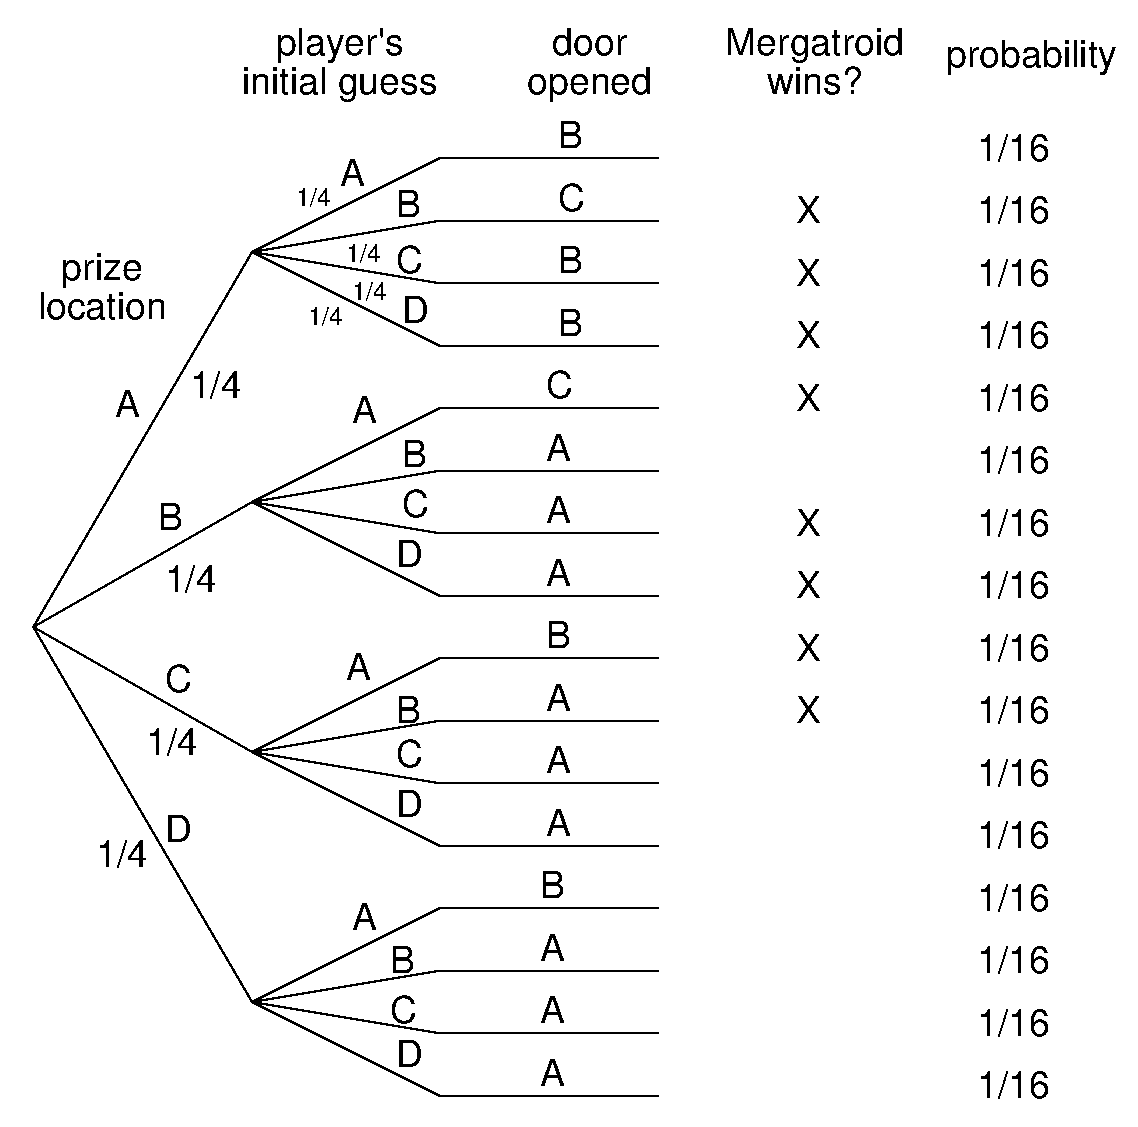
\includegraphics[height=3.5in]{carol}
\end{center}
%
The probability that Mergatroid wins is:
%
\[
\pr{\text{win}} = 8 \cdot \frac{1}{16} = \frac{1}{2}
\]
\end{solution}

\eparts

\end{problem}


%%%%%%%%%%%%%%%%%%%%%%%%%%%%%%%%%%%%%%%%%%%%%%%%%%%%%%%%%%%%%%%%%%%%%
% Problem ends here
%%%%%%%%%%%%%%%%%%%%%%%%%%%%%%%%%%%%%%%%%%%%%%%%%%%%%%%%%%%%%%%%%%%%%

\endinput
